% VIO notes final LaTeX source
\documentclass[11pt]{article}

\usepackage[a4paper,margin=1in]{geometry}
\usepackage{amsmath,amssymb,mathtools,bm}
\usepackage{graphicx}
\usepackage{tikz}
\usetikzlibrary{arrows.meta,positioning,calc,fit}
\usepackage[hidelinks]{hyperref}
\usepackage{algorithm}
\usepackage[noend]{algpseudocode}

\newcommand{\R}{\mathbb{R}}
\newcommand{\SO}{\mathrm{SO}(3)}
\newcommand{\Log}{\mathrm{Log}}
\newcommand{\Exp}{\mathrm{Exp}}
\newcommand{\crossmat}[1]{\left[#1\right]_{\times}}
\newcommand{\norm}[1]{\left\lVert #1 \right\rVert}
\newcommand{\T}{^{\top}}

\title{Visual--Inertial Odometry (VIO) Notes}
\author{Sebastiano Mengozzi}
\date{March 2026}

\begin{document}
\maketitle

\section{Objective function}

We estimate the variables in the active optimization set by minimizing a weighted least-squares cost:
\begin{equation}
J(\mathbf{X}) = \norm{\mathbf{r}_{\mathrm{prior}}}_{\Sigma_{\mathrm{prior}}^{-1}}^2
+ \sum_{(i,j)\in \mathcal{I}} \norm{\mathbf{r}^{\mathrm{imu}}_{ij}}_{\Sigma_{ij}^{-1}}^2
+ \sum_{(i,\ell)\in \mathcal{C}} \norm{\mathbf{r}^{\mathrm{cam}}_{i\ell}}_{\Sigma_{i\ell}^{-1}}^2,
\end{equation}
where \(\norm{\mathbf{r}}_{\Sigma^{-1}}^2 = \mathbf{r}\T \Sigma^{-1} \mathbf{r}\).
The estimate is
\begin{equation}
\hat{\mathbf{X}} = \arg\min_{\mathbf{X}} J(\mathbf{X}).
\end{equation}
where the optimization variables are collected in
\begin{equation}
\mathbf{X} = \left\{\mathbf{x}_i,\, \mathbf{P}_\ell^W\right\},
\end{equation}
and the index sets are:
\begin{itemize}
    \item \(\mathcal{I}\): set of consecutive keyframe pairs \((i,j)\) with an active IMU factor,
    \item \(\mathcal{C}\): set of (keyframe, landmark) pairs \((i,\ell)\) with a valid reprojection observation,
    \item \(\mathbf{x}_i = (\mathbf{R}_i,\mathbf{p}_i,\mathbf{v}_i,\mathbf{b}_{g,i},\mathbf{b}_{a,i})\): state at keyframe \(i\),
    \item \(\mathbf{P}_\ell^W \in \R^3\): position of landmark \(\ell\) in the world frame,
    \item \(\mathbf{r}_{\mathrm{prior}}\): residual encoding information from marginalized states,
    \item \(\mathbf{r}^{\mathrm{imu}}_{ij} \in \R^{15}\): IMU residual between keyframes \(i\) and \(j\),
    \item \(\mathbf{r}^{\mathrm{cam}}_{i\ell} \in \R^{2}\): camera reprojection residual for landmark \(\ell\) at keyframe \(i\),
    \item \(\Sigma_{\mathrm{prior}}, \Sigma_{ij}, \Sigma_{i\ell}\): covariance matrices of the corresponding noise terms.
\end{itemize}

The three terms correspond to: prior information, IMU constraints, and camera reprojection constraints. 
For simplicity, we omit the prior term in the following. 
\\
Intuitively, the prior encodes information from states that 
have been removed from the active window: when the oldest state is marginalized out, its contribution is compressed into 
a prior factor that is carried forward, preserving the information without keeping the full state history. Marginalization 
is thus the process of removing the oldest states while mathematically preserving their information as a prior.

\section{State and conventions}

At keyframe (or image time) \(t_i\), the state is
\begin{equation}
\mathbf{x}_i = (\mathbf{R}_i,\mathbf{p}_i,\mathbf{v}_i,\mathbf{b}_{g,i},\mathbf{b}_{a,i}),
\end{equation}
with
\(\mathbf{R}_i\in \SO\), \(\mathbf{p}_i,\mathbf{v}_i\in\R^3\), and gyro/accelerometer biases
\(\mathbf{b}_{g,i},\mathbf{b}_{a,i}\in\R^3\).
\\
We use the convention that \(\mathbf{R}_i\) maps vectors from the body frame \(B_i\) to the world frame \(W\).
Therefore, \(\mathbf{R}_i\T\) maps vectors from world to body coordinates.
\\
With this convention, all frame transformations in the camera and IMU equations stay consistent.

\section{Camera model and residual}

Let \(\mathbf{P}_\ell^W\in\R^3\) be the position of landmark \(\ell\) in the world frame.
Let the camera extrinsics be \((\mathbf{R}_{CB},\mathbf{p}_{BC}^B)\), where:
\begin{itemize}
  \item \(\mathbf{R}_{CB}\) rotates body-frame vectors into camera-frame vectors,
  \item \(\mathbf{p}_{BC}^B\) is the camera position relative to the body origin, expressed in the body frame.
\end{itemize}
\
Then the landmark coordinates in the body and camera frames are
\begin{align}
\mathbf{P}_\ell^{B_i} &= \mathbf{R}_i\T (\mathbf{P}_\ell^W - \mathbf{p}_i), \\
\mathbf{P}_\ell^{C_i} &= \mathbf{R}_{CB}(\mathbf{P}_\ell^{B_i} - \mathbf{p}_{BC}^B).
\end{align}
\
Using the pinhole model with intrinsic matrix
\begin{equation}
\mathbf{K} =
\begin{bmatrix}
 f_x & 0   & c_x \\
 0   & f_y & c_y \\
 0   & 0   & 1
\end{bmatrix},
\end{equation}
and \(\mathbf{P}_\ell^{C_i}=(x,y,z)\T\), the projected pixel is
\begin{equation}
\hat{\mathbf{u}}_{i\ell} =
\begin{bmatrix}
 f_x x/z + c_x \\
 f_y y/z + c_y
\end{bmatrix}.
\end{equation}
If \(\mathbf{u}_{i\ell}\) is the observed pixel, the camera residual is
\begin{equation}
\mathbf{r}^{\mathrm{cam}}_{i\ell} = \mathbf{u}_{i\ell} - \hat{\mathbf{u}}_{i\ell}.
\end{equation}
\\
The camera factor penalizes the mismatch between the measured image point and the point predicted by the current state \(\mathbf{x}_i\) and landmark estimate \(\mathbf{P}_\ell^W\).

\section{IMU measurement model}

The gyroscope and accelerometer measurements are modeled as
\begin{align}
\boldsymbol{\omega}_m(t) &= \boldsymbol{\omega}(t) + \mathbf{b}_g(t) + \mathbf{n}_g(t), \\
\mathbf{a}_m(t) &= \mathbf{f}(t) + \mathbf{b}_a(t) + \mathbf{n}_a(t),
\end{align}
where
\begin{itemize}
  \item \(\boldsymbol{\omega}(t)\) is the true body angular velocity,
  \item \(\mathbf{f}(t)\) is the true specific force in the body frame,
  \item \(\mathbf{n}_g,\mathbf{n}_a\) are white noise terms.
\end{itemize}
The biases are usually modeled as random walks:
\begin{align}
\dot{\mathbf{b}}_g(t) &= \mathbf{n}_{wg}(t), \\
\dot{\mathbf{b}}_a(t) &= \mathbf{n}_{wa}(t).
\end{align}
\\
The accelerometer does not directly measure world acceleration; it measures specific force in the body frame.

\section{Continuous-time kinematics}

The motion model is
\begin{align}
\dot{\mathbf{R}}(t) &= \mathbf{R}(t)\crossmat{\boldsymbol{\omega}(t)}, \label{eq:Rdot}\\
\dot{\mathbf{v}}(t) &= \mathbf{g} + \mathbf{R}(t)\mathbf{f}(t), \label{eq:vdot}\\
\dot{\mathbf{p}}(t) &= \mathbf{v}(t). \label{eq:pdot}
\end{align}
\\
Here \(\crossmat{\boldsymbol{\omega}(t)}\) denotes the skew-symmetric matrix associated with the angular velocity vector \(\boldsymbol{\omega}(t)\), i.e., the matrix representation of the cross product with \(\boldsymbol{\omega}(t)\).
\\
Equation \eqref{eq:Rdot} describes orientation dynamics, \eqref{eq:vdot} gives the velocity derivative in world frame, and \eqref{eq:pdot} is standard position kinematics.

\section{Role of the IMU}

It is crucial to distinguish two different uses of the IMU data.

\subsection{Role 1: propagating the newest state}
When a new keyframe \(j\) arrives, raw IMU samples between \(t_i\) and \(t_j\) are used to propagate an initial guess for the new state from \(\mathbf{x}_i\) to \(\mathbf{x}_j\).

\subsection{Role 2: building IMU factors in the optimization window}
For every consecutive pair of states \((i,j)\) currently in the active optimization window, the raw IMU samples between \(t_i\) and \(t_j\) are preintegrated into one IMU factor (and stored).
Therefore preintegration is not only used for the newest interval: it exists for all active IMU intervals in the window.
The optimization uses stored IMU factors on all intervals in the current window, not only on the newest state.

\section{Preintegration from raw IMU samples}

Consider one interval \((i,j)\), and let \((\bar{\mathbf{b}}_{g,i},\bar{\mathbf{b}}_{a,i})\) be the bias linearization point.
For each IMU sample \(k\) in that interval, define the bias-corrected quantities
\begin{equation}
\tilde{\boldsymbol{\omega}}_k = \boldsymbol{\omega}_{m,k} - \bar{\mathbf{b}}_{g,i},
\qquad
\tilde{\mathbf{f}}_k = \mathbf{a}_{m,k} - \bar{\mathbf{b}}_{a,i}.
\end{equation}
\\
Using a simple discrete propagation, the preintegrated quantities evolve as
\begin{align}
\widehat{\Delta \mathbf{R}}_{k+1}
&= \widehat{\Delta \mathbf{R}}_k\, \Exp\!\big(\tilde{\boldsymbol{\omega}}_k\,\Delta t_k\big), \\
\widehat{\Delta \mathbf{v}}_{k+1}
&= \widehat{\Delta \mathbf{v}}_k + \widehat{\Delta \mathbf{R}}_k\,\tilde{\mathbf{f}}_k\,\Delta t_k, \\
\widehat{\Delta \mathbf{p}}_{k+1}
&= \widehat{\Delta \mathbf{p}}_k + \widehat{\Delta \mathbf{v}}_k\,\Delta t_k
+ \tfrac{1}{2}\widehat{\Delta \mathbf{R}}_k\,\tilde{\mathbf{f}}_k\,\Delta t_k^2.
\end{align}
with initialization
\begin{equation}
\widehat{\Delta \mathbf{R}}_{ii}=\mathbf{I},
\qquad
\widehat{\Delta \mathbf{v}}_{ii}=\mathbf{0},
\qquad
\widehat{\Delta \mathbf{p}}_{ii}=\mathbf{0}.
\end{equation}
\\
These equations use the raw IMU data and produce the measurement-side quantities \(\widehat{\Delta \mathbf{R}}_{ij},\widehat{\Delta \mathbf{v}}_{ij},\widehat{\Delta \mathbf{p}}_{ij}\) associated with the interval \((i,j)\).

\section{Relative motion implied by the states}

Now consider two states already present in the optimization variables:
\(\mathbf{x}_i\) and \(\mathbf{x}_j\).
From these states alone, we can compute the relative motion they imply:
\begin{align}
\Delta \mathbf{R}^{\mathrm{state}}_{ij} &= \mathbf{R}_i\T \mathbf{R}_j, \\
\Delta \mathbf{v}^{\mathrm{state}}_{ij} &= \mathbf{R}_i\T\left(\mathbf{v}_j - \mathbf{v}_i - \mathbf{g}\,\Delta t_{ij}\right), \\
\Delta \mathbf{p}^{\mathrm{state}}_{ij} &= \mathbf{R}_i\T\left(\mathbf{p}_j - \mathbf{p}_i - \mathbf{v}_i\,\Delta t_{ij} - \tfrac{1}{2}\mathbf{g}\,\Delta t_{ij}^2\right).
\end{align}
\\
These expressions do \emph{not} use raw IMU samples. They are computed only from the current guessed states in the optimizer. They describe the motion encoded by the pair \((\mathbf{x}_i,\mathbf{x}_j)\).

\section{IMU residual}

The IMU factor compares:
\begin{itemize}
  \item the motion preintegrated from raw IMU samples, and
  \item the motion implied by the current state estimates.
\end{itemize}
The residual components are
\begin{align}
\mathbf{r}_{\Delta R,ij}
&= \Log\!\left( \widehat{\Delta \mathbf{R}}_{ij}\T\,\Delta \mathbf{R}^{\mathrm{state}}_{ij} \right), \\
\mathbf{r}_{\Delta v,ij}
&= \Delta \mathbf{v}^{\mathrm{state}}_{ij} - \widehat{\Delta \mathbf{v}}_{ij}, \\
\mathbf{r}_{\Delta p,ij}
&= \Delta \mathbf{p}^{\mathrm{state}}_{ij} - \widehat{\Delta \mathbf{p}}_{ij}, \\
\mathbf{r}_{b_g,ij}
&= \mathbf{b}_{g,j} - \mathbf{b}_{g,i}, \\
\mathbf{r}_{b_a,ij}
&= \mathbf{b}_{a,j} - \mathbf{b}_{a,i}.
\end{align}
Stacking them gives
\begin{equation}
\mathbf{r}^{\mathrm{imu}}_{ij} =
\begin{bmatrix}
\mathbf{r}_{\Delta R,ij} \\
\mathbf{r}_{\Delta v,ij} \\
\mathbf{r}_{\Delta p,ij} \\
\mathbf{r}_{b_g,ij} \\
\mathbf{r}_{b_a,ij}
\end{bmatrix}.
\end{equation}
\\
The IMU residual is therefore the mismatch between two descriptions of the same motion over \((i,j)\): one from measurements, one from the current optimization states.

\section{Time interpretation and sliding-window implementation}

A common source of confusion is the meaning of ``current,'' ``past,'' and ``future.''
In online VIO, the active variable set is usually a sliding window
\begin{equation}
\mathbf{X} = \{\mathbf{x}_{k-m},\mathbf{x}_{k-m+1},\dots,\mathbf{x}_{k}\},
\end{equation}
where \(\mathbf{x}_k\) is the latest state at the current time, and the other states are recent past states.
So \(\mathbf{X}\) is usually a recent piece of the trajectory, not the entire trajectory and not true future states.
\\

The optimizer refines all states currently in the window, including past ones, because new camera and IMU information can improve them.
For example, if
\begin{equation}
\mathbf{X}=\{\mathbf{x}_2,\mathbf{x}_3,\mathbf{x}_4,\mathbf{x}_5\},
\end{equation}
then the active IMU factors are typically
\begin{equation}
\hat z^{\mathrm{imu}}_{23},\qquad \hat z^{\mathrm{imu}}_{34},\qquad \hat z^{\mathrm{imu}}_{45}.
\end{equation}
The newest state \(\mathbf{x}_5\) is initialized by IMU propagation from \(\mathbf{x}_4\), but the optimization uses all active IMU factors in the current window (see Fig.~\ref{fig:active_window}).

\begin{figure}[h!]
\centering
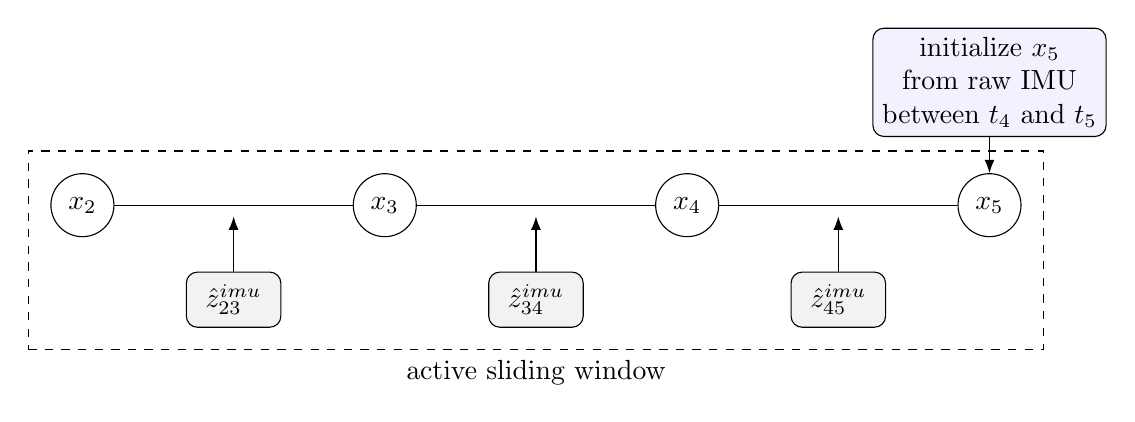
\begin{tikzpicture}[x=2.4cm,y=1.2cm,>=Latex]
  \node[circle,draw,minimum size=8mm] (x2) at (0,0) {$x_2$};
  \node[circle,draw,minimum size=8mm] (x3) at (1.6,0) {$x_3$};
  \node[circle,draw,minimum size=8mm] (x4) at (3.2,0) {$x_4$};
  \node[circle,draw,minimum size=8mm] (x5) at (4.8,0) {$x_5$};

  \node[draw,rounded corners,fill=gray!10,minimum width=1.2cm,minimum height=7mm] (z23) at (0.8,-1.0) {$\hat z^{imu}_{23}$};
  \node[draw,rounded corners,fill=gray!10,minimum width=1.2cm,minimum height=7mm] (z34) at (2.4,-1.0) {$\hat z^{imu}_{34}$};
  \node[draw,rounded corners,fill=gray!10,minimum width=1.2cm,minimum height=7mm] (z45) at (4.0,-1.0) {$\hat z^{imu}_{45}$};

  \draw[-] (x2) -- (x3);
  \draw[-] (x3) -- (x4);
  \draw[-] (x4) -- (x5);

  \draw[->] (z23.north) -- (0.8,-0.12);
  \draw[->] (z34.north) -- (2.4,-0.12);
  \draw[->] (z45.north) -- (4.0,-0.12);

  \node[draw,rounded corners,align=center,fill=blue!5] (init) at (4.8,1.3) {initialize $x_5$\\from raw IMU\\between $t_4$ and $t_5$};
  \draw[->] (init.south) -- (x5.north);

  \node[draw,dashed,fit=(x2)(x3)(x4)(x5)(z23)(z34)(z45),inner sep=8pt,label=below:{active sliding window}] {};
\end{tikzpicture}
\caption{The active window contains recent states and all corresponding IMU factors. The newest state is initialized using raw IMU, while the optimizer uses IMU factors for every active interval.}
\label{fig:active_window}
\end{figure}

\newpage

\section{Pseudo-algorithm}
The newest state is initialized from IMU propagation, but the optimizer refines the full active window using all stored visual and inertial factors.
For simplicity, this exposition omits the explicit marginalization process and prior term generation, though both are essential components of a complete implementation.

\begin{algorithm}[h]
\caption{Keyframe-Based Visual-Inertial Sliding Window Optimization}
\label{alg:vio_sliding_window}
\begin{algorithmic}[1]
\State \textbf{Inpunt:} 
    \Statex \hspace{\algorithmicindent} $\mathcal{X}_{old} = \{x_{k-m}, \dots, x_{k-1}\}$ \Comment{Current sliding window}
    \Statex \hspace{\algorithmicindent} $\mathcal{S}_{k-1 \to k} = \{(\omega_m, a_m)_t\}_{t_{k-1}}^{t_k}$ \Comment{Raw IMU samples}
    \Statex \hspace{\algorithmicindent} $\mathcal{U}_k = \{\mathbf{u}_{i\ell}\}$ and $\mathcal{P} = \{\mathbf{P}_\ell\}$ \Comment{2D detections and 3D landmarks}
    
\State \textbf{Optimization step} $k$:

\Statex \textbf{1. State Initialization}
\State Propagate $x_{k-1}$ using $\mathcal{S}_{k-1 \to k}$ to obtain initial guess $x_k$

\Statex \textbf{2. Window Management}
\State $\mathcal{X} \gets \{x_{k-m+1}, \dots, x_{k-1}, x_k\}$ \Comment{Slide window forward}

\Statex \textbf{3. Visual Residual Computation}
\For{each observation $\mathbf{u}_{i\ell} \in \mathcal{U}_k$}
    \State Compute camera residual $\mathbf{r}^{cam}_{i\ell} = \mathbf{u}_{i\ell} - \pi(x_i, \mathbf{P}_\ell)$ \Comment{Difference from projection model}
\EndFor

\Statex \textbf{4. Inertial Preintegration and Residuals}
\For{each consecutive pair $(i, j) \in \mathcal{X}$}
    \State Compute IMU residual $\mathbf{r}^{imu}_{ij}$ \Comment{Compare state-implied motion with IMU}
    \State Compute covariance $\Sigma_{ij}$ and bias Jacobians $\mathcal{J}_{ij}$
\EndFor

\Statex \textbf{5. Joint Optimization}
\State $J(\mathcal{X}) = \sum \|\mathbf{r}^{cam}_{i\ell}\|^2_{\Sigma_{cam}} + \sum \|\mathbf{r}^{imu}_{ij}\|^2_{\Sigma_{ij}}$
\State $\mathcal{X} \gets \arg\min_{\mathcal{X}} J(\mathcal{X})$ \Comment{Solve via least-squares}

\end{algorithmic}
\end{algorithm}


\newpage

\section{Compact block scheme}

\begin{figure}[h!]
\centering
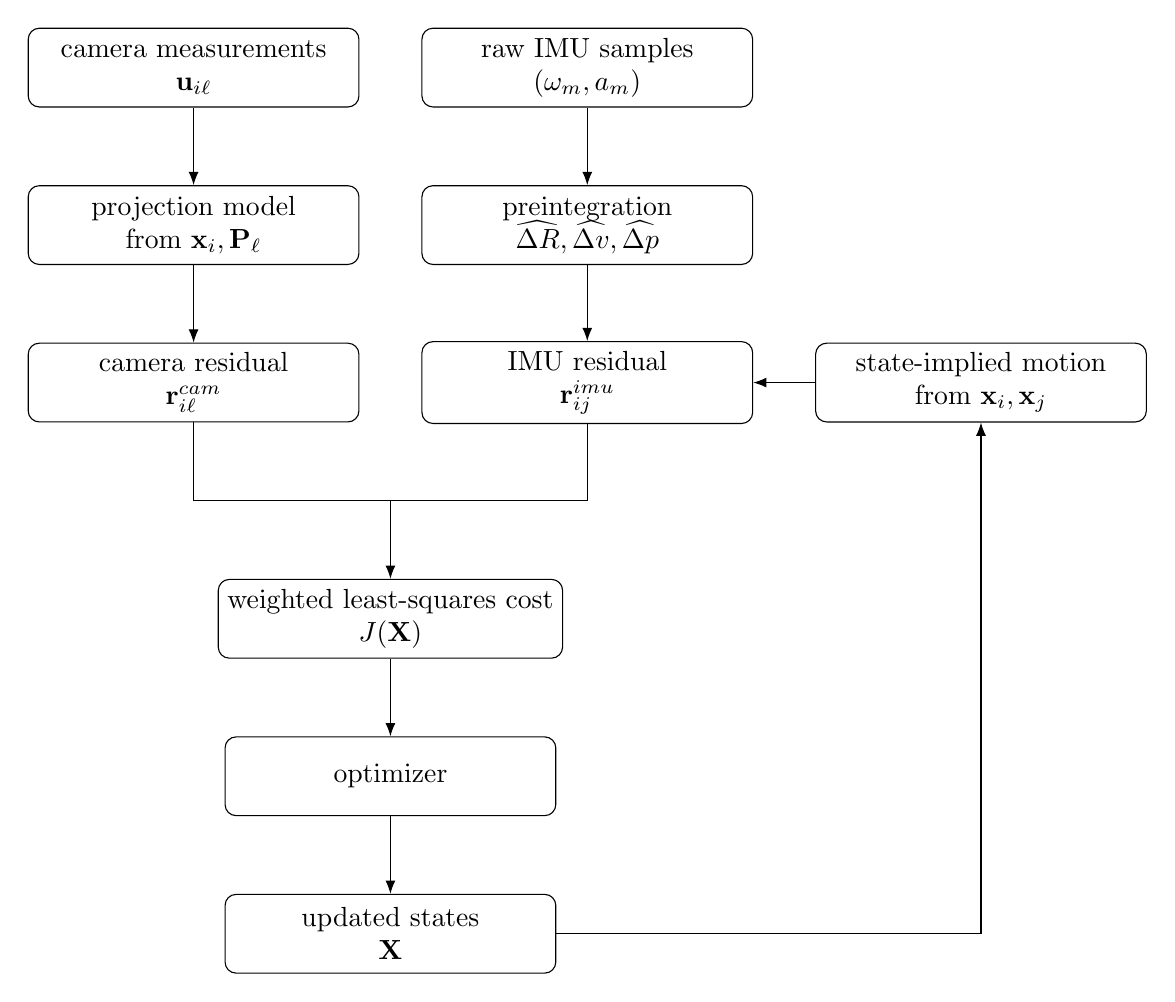
\begin{tikzpicture}[>=Latex]
  \tikzstyle{block}=[draw,rounded corners,minimum width=42mm,minimum height=10mm,align=center]

  % Camera column
  \node[block] (cammeas) at (0,0) {camera measurements\\$\mathbf{u}_{i\ell}$};
  \node[block] (cammodel) at (0,-2) {projection model\\from $\mathbf{x}_i,\mathbf{P}_\ell$};
  \node[block] (camres) at (0,-4) {camera residual\\$\mathbf{r}^{cam}_{i\ell}$};

  % IMU column
  \node[block] (imumeas) at (5,0) {raw IMU samples\\$(\omega_m,a_m)$};
  \node[block] (preint) at (5,-2) {preintegration\\$\widehat{\Delta R},\widehat{\Delta v},\widehat{\Delta p}$};
  \node[block] (imustate) at (10,-4) {state-implied motion\\from $\mathbf{x}_i,\mathbf{x}_j$};
  \node[block] (imures) at (5,-4) {IMU residual\\$\mathbf{r}^{imu}_{ij}$};

  % Bottom chain
  \node[block] (cost) at (2.5,-7) {weighted least-squares cost\\$J(\mathbf{X})$};
  \node[block] (opt) at (2.5,-9) {optimizer};
  \node[block] (out) at (2.5,-11) {updated states\\$\mathbf{X}$};

  % Camera arrows
  \draw[->] (cammeas) -- (cammodel);
  \draw[->] (cammodel) -- (camres);

  % IMU arrows
  \draw[->] (imumeas) -- (preint);
  \draw[->] (preint) -- (imures);
  \draw[->] (imustate.west) -- (imures.east);

% 1. Create a merge point at X=2.5, aligned vertically with the target block's top
\coordinate (merge) at (2.5, -5.5);

% 2. Route the arrows to this merge point
\draw (camres.south) |- (merge);
\draw (imures.south) |- (merge);

% 3. Final arrow from the merge point into the cost block
\draw[->] (merge) -- (cost.north);

  % Optimization chain
  \draw[->] (cost) -- (opt);
  \draw[->] (opt) -- (out);
  \draw[->] (out.east) -| (imustate.south);

\end{tikzpicture}
\caption{Visual and inertial residuals both contribute to the same optimization problem. The IMU branch explicitly compares preintegrated motion from raw measurements with motion implied by the current states.}
\end{figure}

\end{document}
